% !TeX root = ../thuthesis-example.tex

\chapter{绪论}


%
\section{研究背景与意义}

近年来,人工智能技术的发展始终处在快车道,在全球范围内不断取得重大突破,逐渐成为引领性技术。
从统计分析到智能感知再到生成式AI和智能预测,以机器学习为首的人工智能技术持续在不同领域不同任务上发光发热,不断为各行各业带来革命性的转变。
世界各国和主要经济体纷纷加快人工智能战略布局,并相应出台了一系列人工智能发展规划、政策和法律法规。
美国的《国家人工智能研究与发展战略计划》、欧盟的《人工智能法案》、我国的《数字中国建设整体布局规划》和《全球人工智能治理倡议》等一系列战略文件,都明确了人工智能技术的重要性和发展方向,推动着产业界和学术界的技术创新和应用落地。

技术变革的阶段往往也是野蛮生长的阶段,人们关注的焦点大多是如何快速地深化技术,以搏取先发优势和领导者地位。
但当技术面临落地时,工程化、标准化、规模化等方面的诸多挑战开始凸显,制约着其应用推广。
对于机器学习而言,技术增长期常见的“烟囱式”、“手工作坊式”等不成体系的研发模式是造成其应用成本高、管理乱、落地难的重要原因:
一方面,模型研发的工作流程缺乏顶层设计,分工不明确,易出现重复劳动,难以形成有效的团队协作;
另一方面,模型研发过程中产生的资产缺乏统一的存储和管理,资产易流失,经验难传承,难以形成有效的知识沉淀和复用。

\begin{figure}
  \centering
  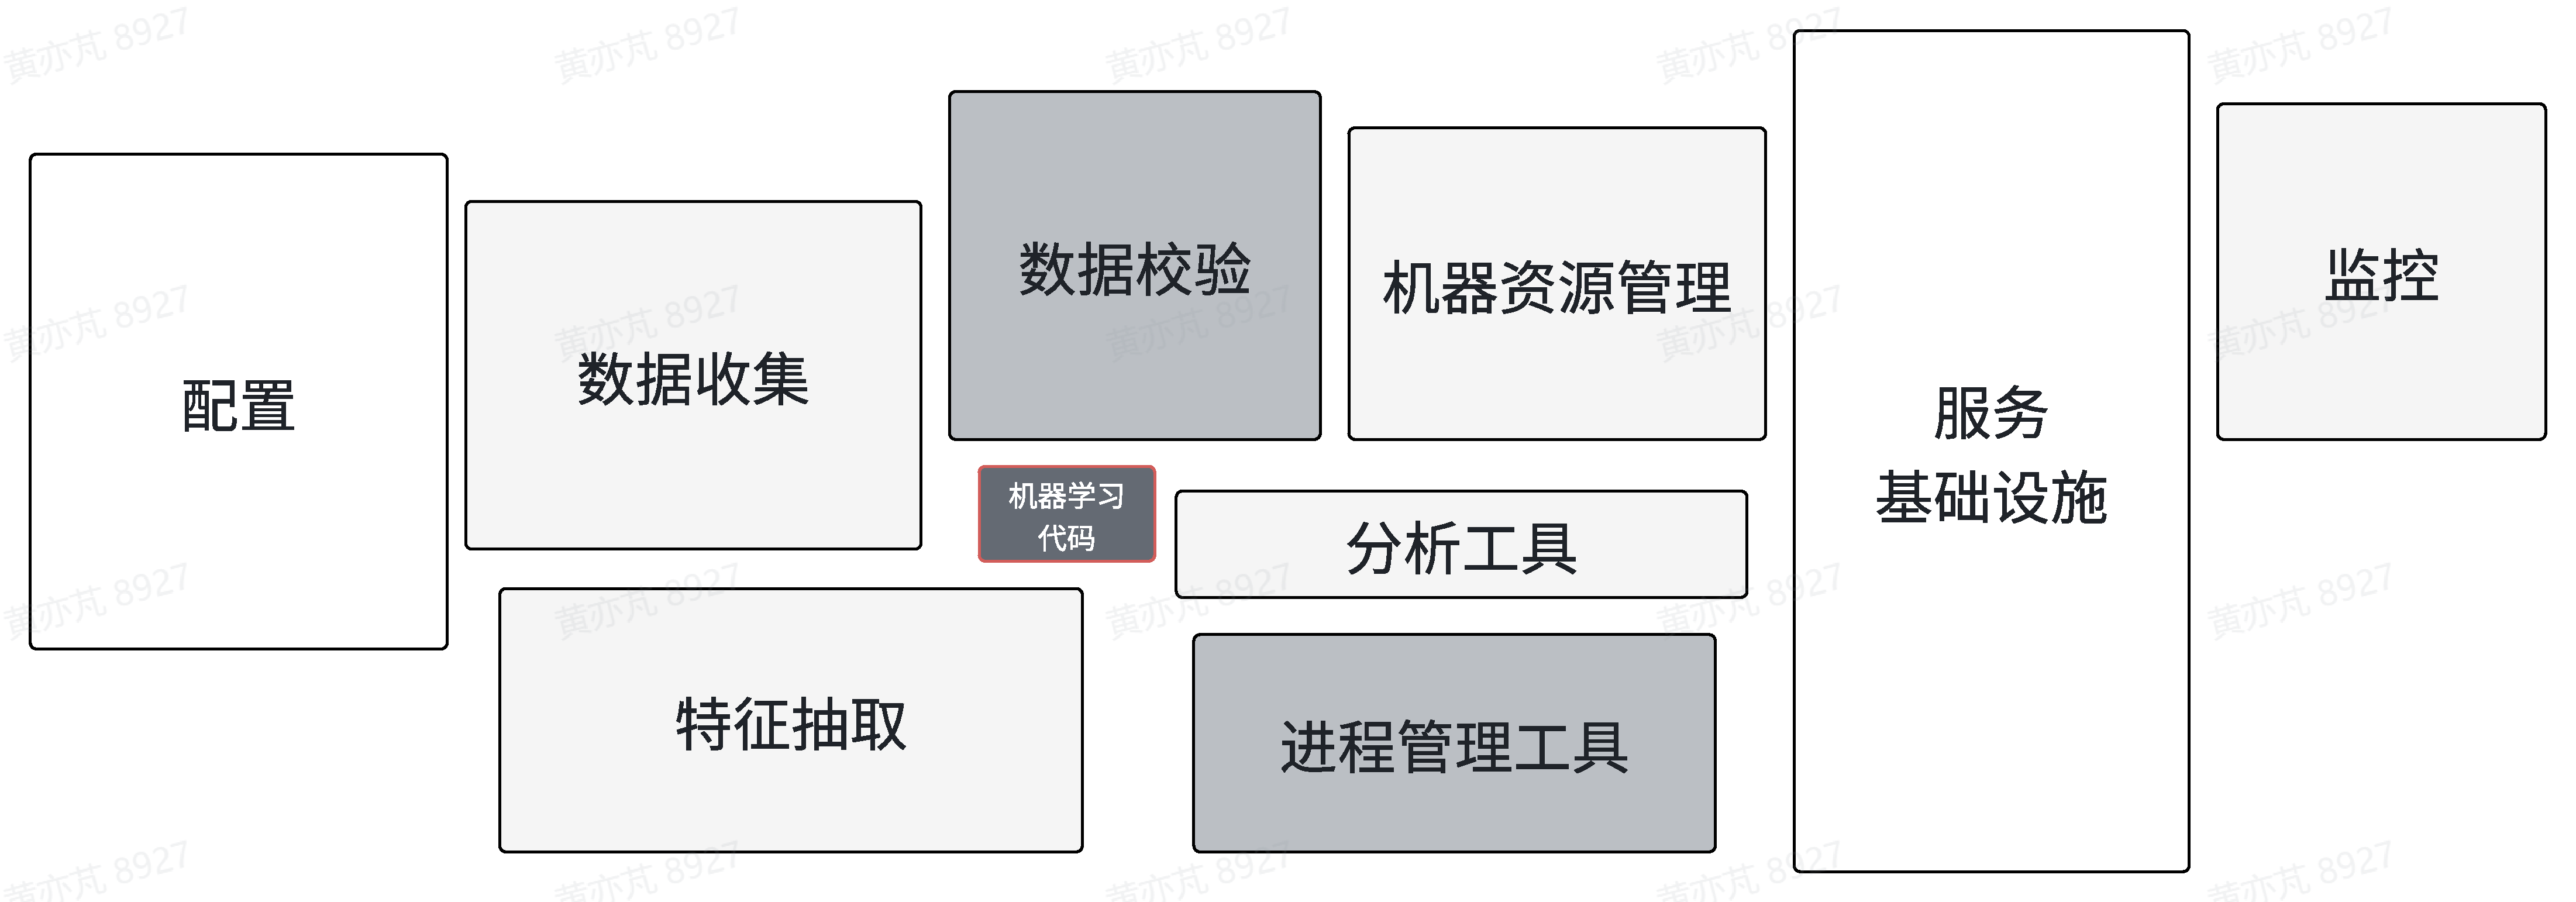
\includegraphics[width=0.98\linewidth]{ml-system-components.pdf}
  \caption{谷歌提出的机器学习系统组成}
  \label{fig:mlcomponents}
\end{figure}

人类的技术发展总是伴随着工程化的进程:从人力种植到机械耕作、从手工制造到工业生产、从编程开发到软件工程等等。
其中的关键是工具手段的出现和演进以及流程的标准化和自动化,以支撑技术的规模化应用。
其核心就是提高生产效率,从而解放生产力,降低生产成本,提高产品质量。
在机器学习领域,工程化的进程也是必然的,也是迫切的。
正如谷歌在机器学习系统设计的奠基性理论研究中所提出的,真实世界的机器学习系统中包含广阔而复杂的工程化基础设施,机器学习代码只是系统中很小的一部分,如图\ref{fig:mlcomponents}。
在模型核心技术研发的层面上,数据准备、算法开发、模型训练、模型评估等环节需要工具手段的辅助,以提高研发效率和模型性能;
在模型应用落地的层面上,模型部署、模型监控、流程自动化、业务应用集成等环节更需要工程化的系统软件支撑,以保证应用的稳定性、可靠性和可维护性。
因此,构建体系化的云原生机器学习平台,以工程手段来解决机器学习研发的相关挑战,是当前机器学习技术发展的必然趋势,也是本文研究的重要意义。

【与软件工程的不同】
模型结构复杂、训练数据多、参数量大、随机性强

【为什么云原生】

需要注意的是,一些文献中将PyTorch、TensorFlow等机器学习计算框架称为机器学习平台,易与本文的研究对象混淆。
本文研究的机器学习平台是指支撑机器学习研发和应用的软件工具系统,依托于硬件基础设施(或称硬件平台,亦与本文中的平台不同),支持在平台中使用PyTorch、TensorFlow等机器学习计算框架进行模型训练、推理等计算作业。


%
\section{国内外研究现状}

机器学习平台的研究和实践已经有了多年的积累,学术界在数据分析与MLOps理论方法和相关系统研究方面均形成了一些高水平的成果,产业界近些年也涌现了一批成熟的平台产品。
下面将从理论方法、系统研究和平台产品3个方面对国内外的研究现状进行梳理。

\subsection{理论方法}

大数据挖掘领域最经典的方法论是跨行业数据挖掘标准过程(Cross-Industry Standard Process for Data Mining, CRISP-DM)\cite{Wir00},它将数据挖掘过程分为6个阶段:业务理解、数据理解、数据准备、建模、评价和部署,并提出了业务理解与数据理解之间以及数据准备与建模之间的反馈循环,充分抽象了在实际进行大数据挖掘时最常需要迭代的几个步骤,同时也提出了从评价回到业务理解的大循环,体现了以评价指标为导向的数据挖掘解决方案的整体迭代。
其实,不仅限于标题中的数据挖掘,CRISP-DM在更为宏观的大数据分析方面都发挥着极为重要的指导作用,为包括人工智能分析在内的数据分析人员提供了一套标准的流程框架,是后续更现代的人工智能工程化方法论的基石。

Amershi等人\cite{Ame19}特别针对机器学习中的软件工程方法进行了研究。
通过对微软多个产品团队的工程师进行访谈和问卷调查,作者总结了机器学习九阶段工作流,涵盖模型需求分析、数据收集、数据清洗、数据标注、特征工程、模型训练、模型评价、模型部署和模型监控。
与CRISP-DM的多项反馈循环类似,作业通过特征工程与模型训练之间的反馈回路强调了特征工程对于模型效果的重要性,并指出了在模型评价和模型监控阶段均可分别根据离线指标和在线指标返回工作流之前的任何步骤进行迭代。
此外,作者提出了多项机器学习工程化的最佳实践,如模型和数据版本控制、人机混合协作的模型评估等,并设计了AI过程成熟度模型,用于帮助团队系统评估和优化其ML工作流。

近年来,人工智能研发人员逐渐意识到工程化在应用落地中的重要性,产业界基于软件工程领域的DevOps框架延申出了机器学习持续交付(CD4ML)理念,进而演化成了机器学习加DevOps的MLOps概念,并逐渐被学界和业界广泛接受,成为人工智能工程化方面最流行的体系框架之一。

实际上,MLOps的奠基之作被普遍认为是Sculley等人的论文\cite{Scu15}。作者虽未明确提出MLOps的概念,但对于机器学习系统落地的挑战进行了深入的探讨,其中有多个观点发人深省。第一,作者认为开发和部署机器学习系统相对快速且成本低廉,但后期持续维护这些系统既艰难又昂贵。第二,并非所有技术负债都是不好的,但所有技术负债都有代价。第三,相比传统的软件系统,机器学习系统更易出现技术负债,因为除了传统软件会面临的系统维护问题以外,还会面临很多机器学习特有的问题,例如:1)机器学习模型的黑盒化过于严重,其中可能含有大量假设、硬编码等不可维护的逻辑;2)机器学习模型与数据和特征的耦合度过高,一旦数据或特征当中发生一点微小的变化都需要重新生成模型;3)机器学习模型研发过程中包含大量的胶水代码,导致需要额外工程化。第四,企业应当推崇科学研究与工程融合并重的文化,使研发人员更加关注功能简化、增强复现能力、系统稳定性、监控等方面,通常这是偿还机器学习系统技术负债的唯一途径。最后,作者在文中着重提出可维护的机器学习(maintainable ML)核心理念,旨在强调为了微小的模型效果提升而大幅增加系统复杂度是不可取的,为MLOps提供了坚实的理论基础。

MLOps框架下还在持续涌现理论方法的相关研究。
在实际的研发工作当中,模型开发过程难复现、实验程序难复用等问题频繁出现,导致大量的重复劳动,研发可持续性较差。
Fursin等人\cite{Fur16}提出了一套模型研发产出的标准框架,规定了环境、算法、程序、流水线等相关内容的定义方式,研发人员可基于此形成研发项目数据库,支撑研发过程中产生的组件、工具、流程的复用,为团队协作提供基础,进而保障研发的可持续性。
为了帮助企业更系统地采用MLOps,John等人\cite{Joh21}提出了一个MLOps框架和成熟度模型,以支持企业评估其MLOps实施阶段,并强调了数据管理和模型监控的必要性。
Mäkinen等人\cite{Mak21}通过对331名数据科学家的调研分析,揭示了MLOps在模型重训练和数据管理中的关键作用,但指出复杂性和成本仍是主要障碍。
Symeonidis等人\cite{Sym22}对MLOps的定义、工具和实施挑战进行了系统综述,指出MLOps的核心在于实现从数据处理到模型管理的自动化,帮助团队跨部门协作并提升部署效率。
进一步,Kreuzberger等人\cite{Kre22}提出了一个统一的MLOps架构模型,结合工具分析和专家访谈,从理论上梳理了MLOps的关键组件和功能模块。
Testi等人\cite{Tes22}则建立了一个详细的分类体系和方法论,将MLOps按功能模块进行划分,以帮助ML团队根据项目需求选择适合的管理工具和实施步骤。

\subsection{系统研究}

针对机器学习应用落地的难题,一些研究工作体现在端到端的机器学习平台上\cite{Bay17, Sal18},机器学习模型的研发只是其中的一个环节。
平台的功能覆盖数据、模型训练和验证、应用部署和监控等方面,期望打通从数据接入到业务应用运维的机器学习完整工作流,满足机器学习应用快速上线并形成稳定服务的需求。
追求落地固然是机器学习技术的主要目标,但从根源上,如何使机器学习研发更高效是亟待突破的首要方向,将会对应用落地带来诸多裨益。

Kumar等人\cite{Kum16}将传统机器学习的模型开发过程抽象成特征工程、算法选择和参数调优等3项关键步骤,统称为“模型选择”(Model Selection),并基于此概念提出一种模型选择管理系统框架,包括声明式实验构建、运行时计算优化、模型来源管理与分析等功能,支撑高效的机器学习实验。
Tsay等人\cite{Tsa22}提出了人工智能实验数据库,着重针对研发过程可复现性问题,通过对实验元信息的建模、抽取和关联,聚焦实验产物及其生成过程的完整详细信息,保障从数据处理到模型实验的复现。
同样在研发过程方面,Sridhar等人\cite{Sri18}提出了模型治理的概念及相关系统,覆盖了机器学习模型开发与部署中的模型血统梳理、可复现性、审计、伸缩等需求,旨在帮助研发人员明确模型的产生路径及其在生产环境中的用途和效果,从而更好地复现研发方案、诊断实验过程中存在的问题。

Vartak等人\cite{Var16}提出一种模型管理系统,以代码侵入的方式对实验进行跟踪,并对模型进行统一存储和索引,为用户提供共享、查询、分析等功能,帮助研发人员梳理模型研发过程、找寻规律并建立整体视角。
Schelter等人\cite{Sch17}则提出一种非侵入式模型跟踪方法,可针对一些机器学习框架自动进行实验记录,并提取出数据集、超参数、模型等机器学习常见资产的元信息,支撑实验的对比和复现以及模型血统分析。
Miao等人\cite{Mia17}针对深度学习模型研发提出了一套模型生命周期管理平台,更多地关注了模型快速迭代过程中的版本控制以及模型的社区式共享机制,并搭配了一种领域专用语言用以高效地检索和查询平台中的模型资产。
此外,该平台内置了一套模型来源管理模块,以图数据库的形式帮助用户记录、管理和梳理深度学习模型开发的过程。

许多研究专注于将MLOps应用于特定的行业和场景中,以提升模型的性能和系统的可扩展性。
在药物发现方面,Spjuth等人\cite{Spj21}提出了结合云计算的MLOps方案,以支持大型药物数据集的处理,优化了模型的可重现性。
Granlund等人\cite{Gra21a}在多组织环境中实施MLOps,揭示了数据共享和隐私管理的挑战,特别是在跨组织合作中引入了有效的合规性机制)。
同时,Granlund等人\cite{Gra21b}展示了医疗设备中合规性驱动的MLOps实施,提供了从ML实验到认证医疗产品的完整管道管理流程。
Gürses-Tran和Monti\cite{Gur22}在电力系统中应用MLOps,利用智能化工具对电力负载进行预测,展示了MLOps在处理不确定性能源方面的价值。

\subsection{平台产品}

产业界近些年也涌现了一批实验跟踪与模型管理的系统或平台\cite{wandb, neptuneai, huggingface},在模型资产管理和团队协作上的实践经验对模型研发管理系统的学术研究具有指导意义。

表\ref{tab:platforms}对比了国内外几个典型的机器学习平台产品,包括Weights \& Biases、SageMaker、Hugging Face、飞桨BML、机器学习PAI、KubeFlow、OpenPAI、MLflow和Polyaxon等。

\begin{landscape}
\begin{table}[ht]
  \centering
  \caption{国内外机器学习平台产品对比}
  \begin{tabularx}{\linewidth}{ccXXX}
  \toprule
  产品名称 & 产品类型 & \multicolumn{1}{c}{功能} & \multicolumn{1}{c}{智能性} & \multicolumn{1}{c}{优势} \\
  \midrule
  Weights \& Biases & 国外商用 & 实验跟踪和版本控制;模型性能监控和可视化;超参数优化 & 支持自动化实验比较、超参数优化,更有效地管理和改进模型 & 强大的实验管理和结果可视化能力;社区和团队协作功能 \\
  SageMaker & 国外商用 & 端到端的机器学习开发环境;数据预处理和模型优化工具 & 集成了自动化模型优化和调参功能,支持多种模型部署方式和扩展 & 丰富的算法和模型选择;高度可扩展的基础设施;AWS生态系统 \\
  Hugging Face & 国外社区 & Transformer和预训练模型共享使用;社区驱动的开放平台 & 以Transformer模型为基础,提供易用的API和预训练模型 & 大规模模型和数据集的开放共享;简单易用的API和工具 \\
  飞桨BML & 国内商用 & 端到端的AI解决方案;多种算法和模型的集成;数据安全和隐私保护 & 整合百度的AI技术和云服务,支持大规模数据处理和深度学习 & 强大的数据处理能力;垂直行业中的深度应用经验 \\
  机器学习PAI & 国内商用 & 机器学习资源管理和调度;数据处理和建模的智能化支持 & 整合阿里的AI技术和云服务,支持弹性计算和高效部署 & 完善的生态系统;深度整合大数据计算能力;行业应用实践 \\
  KubeFlow & 开源 & 在Kubernetes上部署和管理机器学习工作流 & 提供灵活的工作流编排和自动化部署功能 & 云原生和容器化支持;强大的自动化机器学习流程 \\
  OpenPAI & 开源 & 弹性的机器学习资源管理和调度;多种框架和工具的支持 & 提供高度可扩展性和灵活的部署选项 & 微软生态系统;大规模分布式计算;开放和灵活的架构设计 \\
  MLflow & 开源 & 管理机器学习生命周期;支持实验追踪和协作 & 丰富的API和界面,支持多种机器学习框架和云平台集成 & 多种机器学习框架的集成;强调实验复现和模型管理的价值 \\
  Polyaxon & 开源 & 支持机器学习的自动化和复现;资源管理和分布式训练的支持 & 提供了灵活的实验追踪和资源管理功能 & 支持多云环境和本地部署;提供可视化和可扩展的功能集成 \\
  \bottomrule
  \end{tabularx}
  \label{tab:platforms}
\end{table}
\end{landscape}

国外商用平台如Weights \& Biases和SageMaker注重实验管理和自动化优化,前者以实验跟踪、模型性能监控和可视化等功能为核心,后者则通过端到端开发环境和与AWS深度集成的基础设施提供了全面的机器学习支持。Hugging Face作为国外开源社区的代表,专注于Transformer模型及其相关生态的开放共享,以易用的API和工具推动自然语言处理领域的快速创新。

相比之下,国内平台如百度的飞桨BML、阿里巴巴的机器学习PAI和华为的ModelArts,分别依托百度云、阿里云和华为云的技术生态,强调数据安全、隐私保护以及与云计算和大数据的深度结合。
飞桨BML在支持大规模数据处理的同时,整合了百度的AI算法资源,为垂直行业提供了丰富的应用案例。
机器学习PAI则通过智能资源调度和开放算法市场的方式,进一步提升了平台的弹性和行业实践能力。

在开源平台方面,Kubeflow、MLflow、Polyaxon和OpenPAI表现出各自的技术特色。
Kubeflow基于Kubernetes,提供了高扩展性和自动化的机器学习工作流管理。
OpenPAI通过开放的资源管理和任务调度能力,支持工业级AI训练需求。
MLflow以其轻量化和开放性著称,专注于模型实验、部署和版本管理。
Polyaxon则擅长分布式训练和多框架集成,优化实验管理效率。
这些开源平台共同为开发者提供了灵活高效的工具,以应对复杂的机器学习任务。

在智能性方面,国外平台更倾向于通过自动化和容器化技术优化工作流管理与模型开发,而国内平台则结合本地场景需求,在数据安全、资源高效利用以及行业适配性上展现优势。
从功能和优势上看,国外平台通过开放性和生态系统的支持,推动技术的广泛应用;国内平台则依托自身在行业积累和本地技术适配上的实力,为特定场景提供定制化的解决方案。


%
\section{研究内容与主要贡献}

针对机器学习研发过程中存在的工作流程缺乏顶层设计、资产缺乏统一管理等研发管理问题,本文从工程化的角度出发,在体系架构、关键技术和系统设计实现等方面研究如何构建一套云原生机器学习平台,为模型研发团队输出体系化、标准化、规模化的机器学习研发作业和管理能力,并提供覆盖数据开发、模型开发、模型训练、模型调整、模型部署、模型服务等机器学习研发生命周期核心环节的工具手段,提高研发效率和模型性能,为机器学习应用落地提供有力支撑。

本文的主要贡献有以下几方面:
\begin{itemize}
  \item 在体系架构方面,本文按照能力体系、功能体系、数据体系、技术体系和交互体系五个维度展开论述,逐级细化剖析机器学习平台的形态,明确平台的能力边界和组成关系,为平台的设计和实现提供指导;
  \item 在关键技术方面,本文从云原生系统相关技术和机器学习相关技术两个角度进行研究,分别探讨了云原生系统的容器化、资源池化、存储等技术在机器学习平台中发挥的作用和应用价值,以及机器学习模型的训练、调优、部署等方面的核心技术点的背景问题和技术原理;
  \item 在系统设计方面,本文提出了Anylearn大数据机器学习研发管理系统的设计方案,并阐述了实际线上长活环境的运行情况和真实科研用户的使用案例,验证了系统的可行性和有效性。
\end{itemize}


%
\section{本文结构安排}

本文围绕研究内容的体系架构、关键技术和系统实现三方面进行论述,后续章节安排如下:第2章研究机器学习平台的体系架构,包括能力体系、功能体系、数据体系、技术体系和交互体系;第3章研究机器学习平台的关键技术,包括云原生系统相关技术和机器学习相关技术;第4章研究机器学习平台的系统设计实现,包括Anylearn大数据机器学习研发管理系统的使用场景、系统设计、线上环境运行情况和用户使用案例;第5章总结全文,展望未来工作。  
